\documentclass[journal]{IEEEtran}

\usepackage{cite}
%\usepackage{algorithmic}
\usepackage{fixltx2e}
\usepackage{url}
\usepackage{graphicx}
\usepackage{float}
\usepackage{amsmath}
\usepackage[]{algorithm2e}



\floatstyle{ruled}
\newfloat{program}{h}{lop}
\floatname{program}{Code}


%\pagestyle{empty}
\usepackage[latin1]{inputenc}
\usepackage{subfig}


%-------------------------------------------------------------------------
% Use a small font for the verbatim environment
\makeatletter  % makes '@' an ordinary character
\renewcommand{\verbatim@font}{
  \ttfamily\footnotesize\itshape\catcode`\<=\active\catcode`\>=\active }
\makeatother % makes '@' a special symbol again
%-------------------------------------------------------------------------
%

\frenchspacing

\sloppy

\pagestyle{empty}


% correct bad hyphenation here
\hyphenation{op-tical net-works semi-conduc-tor}


\begin{document}


\title{Massively Parallel Processing of Deep Neural Networks with Spark: The MareNostrum Experience}

% author names and IEEE memberships
% note positions of commas and nonbreaking spaces ( ~ ) LaTeX will not break
% a structure at a ~ so this keeps an author's name from being broken across
% two lines.
% use \thanks{} to gain access to the first footnote area
% a separate \thanks must be used for each paragraph as LaTeX2e's \thanks
% was not built to handle multiple paragraphs
%

%\author{
%        Ruben~Tous,	
%	Jordi~Torres,
%	Eduard Ayguad\'e
%                       
%\thanks{Ruben Tous, Jordi Torres and Eduard Ayguad\'e are with the Barcelona Supercomputing Center (BSC) and the Universitat Polit\`ecnica de Catalunya - BarcelonaTech (UPC), Barcelona, Spain}
%}

\author{
		(authorship information omitted for blind review)

%\author{
%		Leonel~ Cruz,
%        Ruben~Tous,
%        Beatriz~Otero,
%        Mouna~Makni 
                       
%\thanks{Leonel Cruz, Ruben Tous, Beatriz Otero and Mouna Makni are with the Universitat Polit\`ecnica de Catalunya - BarcelonaTech (UPC), Barcelona, Spain}
}


% The paper headers
%\markboth{IEEE Multimedia,~Vol.~X, No.~X, Month~2008}%
%{Shell \MakeLowercase{\textit{et al.}}: Bare Demo of IEEEtran.cls for Journals}
% The only time the second header will appear is for the odd numbered pages
% after the title page when using the twoside option.
%
% *** Note that you probably will NOT want to include the author's ***
% *** name in the headers of peer review papers.                   ***
% You can use \ifCLASSOPTIONpeerreview for conditional compilation here if
% you desire.


% make the title area
\maketitle\thispagestyle{empty}


\begin{abstract}
Deployment of a distributed deep learning technology stack on a large parallel system is a very complex process, involving the integration and configuration of several layers of both, general-purpose and custom software. The details of such kind of deployments are rarely described in the literature. This paper presents the experiences observed during the deployment of a technology stack to enable deep learning workloads on MareNostrum, a petascale supercomputer. The components of the chosen layered architecure are described and the performance and scalability of the resulting system is evaluated. This is followed by a discussion about the impact of different configurations including parallelism, storage and networking alternatives, and other aspects related to the execution of deep learning workloads on a traditional HPC setup. The derived conclusions should be useful to guide similarly complex deployments in the future.

%https://experts.illinois.edu/en/publications/deploying-a-large-petascale-system-the-blue-waters-experience
\end{abstract}

% Note that keywords are not normally used for peerreview papers.
%\begin{IEEEkeywords}
%TODO
%\end{IEEEkeywords}


%Paper Torres
%https://upcommons.upc.edu/bitstream/handle/2117/107501/Scaling+a+Convolutional+Neural+Network+for.pdf
\section{Introduction}

\IEEEPARstart{O}{}
Over the past several years, deep neural networks (DNNs) have proven to be an incredibly effective tool for a variety of problems, from computer vision, speech recognition or natural language processing. Their number of parameters and complexity, and the size of the training datasets, have quickly grown, leading to be a first class workload for HPC (High-Performance Computing) infraestructures. However, enabling deep learning workloads on a large parallel system is a very complex process, involving the integration and configuration of several layers of both, general-purpose and custom software. The details of such kind of deployments are rarely described in the literature. This paper presents the experiences observed during the deployment of a technology stack to enable deep learning workloads on a real-world, petascale, HPC setup, the MareNostrum supercomputer. 

The goal of the deployment is to be able to take profit of the computation resources provided by MareNostrum (almost 50K cores and more than 100TB of aggregated RAM) for training DNNs. Nowadays, the usage of GPUs has proven to be the more efficient alternative to train neural networks, speeding up common operations such as large matrix computations \cite{DBLP:conf/isca/LeeKCDKNSSCHSD10, conf/ipps/Fujimoto08}. As their price, performance and energy efficiency improves, GPUs are gaining ground in HPC (both in special-purpose systems and in hybrid general-purpose supercomputers). However, there are still many systems, such as MareNostrum, that continue to use conventional CPUs, as they provide a better overall performance-energy-cost trade-off when used for heterogeneous compute-intensive workloads. 

The key element of the deployed layered architecure is Apache Spark \cite{spark}. In order to isolate machine-learning applications from the particularities of MareNostrum, Spark is usually used as an intermediate layer (not only in MareNostrum, \cite{wang2014} does the same on a Cray X-series supercomputer). The deployment of Spark-enabled clusters over MareNostrum is not trivial, it has required the development of a specific interoperability layer that we call Spark4MN, which will be explained later. On top of this stack (Marenostrum, Spark4MN and Spark) we place a deep learning specific layer, DL4J. DL4J, that is written in Java and has a direct integration with Spark, enables distributed training of deep neural networks through a synchronous data parallelism method. 

These four elements (DL4J, Spark, Spark4MN and MareNostrum) have been integrated enabling to efficiently train deep neural networks over thousands of cores. Apart from the deployment details, the challenge is scalability and proper configuration. Simply running on many cores may yield poor benefits or even degraded performance due to overheads. We deal with this issue and we aim to make the first step towards systematic analysis of the several parameters and optimized configuration.

In order to evaluate the performance and scalability of the proposed software stack on MareNostrum, we have experimented with different workloads and different deployment setups (number of nodes, parallelism configuration, etc.). Through the following sections we explain the different components of the deployment in more detail. Then, we discuss the performed experiments and the obtained results, aiming to shed light onto the parameters that have the biggest impact and their effective configuration. We provide insights into how the job configuration on a traditional HPC setup can be optimized to efficiently run this kind of workloads. The derived conclusions should be useful to guide similarly complex deployments in the future.

%http://onlinelibrary.wiley.com/doi/10.1002/cpe.3850/full
%AlexNet for ImageNet classification (IM)

%https://arxiv.org/pdf/1609.06870.pdf
%AlexNet, GoogLeNet, 

%%%%%%%%%%%%%%%%%%%%%%%%%%%%%%%%%%%%%%%%%%%
\section{Related Work}
%%%%%%%%%%%%%%%%%%%%%%%%%%%%%%%%%%%%%%%%%%%
\label{sec:rw}

Several works have addressed the execution of deep learning workloads on large specific purpose clusters (e.g. \cite{DBLP:journals/corr/abs-1708-02983}), usually involving nodes equiped with GPUs. Deployments over general-purpose HPC systems are less common, and their details are rarely described in the literature. The work described in \cite{DBLP:conf/sc/KeuperP16} analyzes the main bottlenecks of distributed DNNs SGD-based training. The authors conclude that the issue is quickly turning into a vastly communication bound problem which is severily limiting the scalability in most practical scenarios. In \cite{DBLP:journals/corr/abs-1708-05256} authors present a Caffe-based approach to execute deep learning workloads on a contemporary HPC system equiped with Xeon-Phi nodes. They use the Intel distribution of Caffe, that improves Caffe performance when running on CPUs. Authors report to be able to scale the training of a model up to almost 10K nodes, demonstrating that deep learning can be optimized and scaled effectively on many-core, HPC systems. Our approach attempts to overcome the complexity of a direct deployment such as this by relying on an intermediate layer, Apache Spark. In addition to reduce the deployment costs, our approach enables a systematic tuning of the different configuration parameters, both at application level and at infraestructure level. Other works have followed a similar approach but for other kind of workloads. In \cite{michael2014}, authors describe a framework to enable Hadoop workloads on a Cray X-series supercomputer. In \cite{wang2014}, the performance of Spark on an HPC setup is investigated. This work studies the impact of storage architecture, locality-oriented scheduling and emerging storage devices. In \cite{jha2014}, the authors compare the performance of traditional HPC setups against Hadoop-like frameworks over clusters of commodity hardware with respect to the processing of data-intensive workloads. 


%%%%%%%%%%%%%%%%%%%%%%%%%%%%%%%%%%%%%%%%%%%
\section{Deep Neural Networks}
\label{sec:spark}
%%%%%%%%%%%%%%%%%%%%%%%%%%%%%%%%%%%%%%%%%%%
%https://github.com/davidstutz/seminar-neural-networks/blob/master/network-training.tex

Deep neural networks (DNNs) are layered compositional models that enable learning representations of data with multiple levels of abstraction. State-of-the-art DNNs include many variants, specialized in different domains (convolutional deep neural networks, recurrent neural networks, etc.). DNNs are usually trained by using iterative, gradient-based optimizers (typically minibatch SGD) that drive a non-convex cost function to a local minima. In every iteration step we use information about the gradient $\nabla E$ at the current point. In iteration step $[t + 1]$ the weight update $\Delta w[t]$ is determined by taking a step ($\gamma$ is the learning rate) into the direction of the negative gradient at position $w[t]$ such that (in the case of stochastic training):
\begin{align}
\Delta w[t] = - \gamma \frac{\partial E_n}{\partial w[t]}
\end{align}
State-of-the-art networks have a huge number of weights $W$ and the core computation in their training is dominated by dense linear algebra. DNNs training on a single node involves several software and hardware layers. At the top of the stack there is normally a deep learning framework such as DL4J, TensorFlow, Torch, etc. (there may be even an upper layer such as Keras). Below, the framework relies on an underlying numerical library such as NVIDIA's cuDNN or Intel's MKL. Finally, the models are usually trained on NVIDIA GPUs or Intel's Xeon Phi processors. 

When trained on multiple nodes, there are two complementary aproaches. One the one hand, there is data parallelism, an approach in which examples within a batch are divided among the available nodes. Each node stores a complete copy of the model. On the other hand, there's model parallelism, that partitions the model itself by assigning the parameters (and computation) of different layers of the network to different nodes. Focusing on data parallelism, it can be done synchronously or asynchronously. With the synchronous method we wait all the workers to finish before averaging their resulting weight updates. With the asynchronous method we allow the updates to be applied as soon as they are computed. This way we can potentially gain higher throughput, but depending on the infraestructure status we can have the {\it stale gradient problem}. By the time a slow worker has finished its calculations based on a given state of the model, the model may have been updated a number of times and the outdated update may have a negative impact. In this work we focus on synchrounous data parallelism beause it is the only one supported by DL4J over Spark.
%http://engineering.skymind.io/distributed-deep-learning-part-1-an-introduction-to-distributed-training-of-neural-networks

%http://joerihermans.com/ramblings/distributed-deep-learning-part-1-an-introduction/

%%%%%%%%%%%%%%%%%%%%%%%%%%%%%%%%%%%%%%%%%%%
\section{DL4J}
\label{sec:spark}
%%%%%%%%%%%%%%%%%%%%%%%%%%%%%%%%%%%%%%%%%%%
%From https://deeplearning4j.org/spark
DL4J (or Deeplearning4j) is a computing framework written for Java with wide support for deep learning algorithms. DL4J provides distributed parallel versions (both for GPUs and CPUs) of the algorithms that integrate with Apache Hadoop and Spark. In order to achieve distributed network training over Spark, DL4J applies parameter averaging. Training data is divided into a number of splits. Each split is in turn divided into a number of minibatches. At each iteration all the minibatches of one data split are processed in parallel by the available Spark workers. All the resulting parameter updates are averaged and returned to the Spark master. There are several parameters that must be adjusted to optimize training time. These include, but are not limited to, minibach size (number of examples for each parameter update in each worker), averaging frequency (too low averaging periods may imply too networking overhead), prefetching (how many minibatches a worker must prefetch to avoid waiting for the data to be loaded), repartitioning strategy (when and how to repartition data to keep the partitions balanced and the proper level of parallelism, and data locality. 

In addition to properly configure DL4J, in some cases it's also necessary to adjust some Spark default parameters to fit the particularities of a deep learning workload. Deep learning is computationally intensive, and hence the amount of computation per data partition is relatively high. Spark default locality level (when does it make sense to await for a executor closer to the data to become free) needs to be set to zero, as computation time will allways outweigh any network transfer time.  

\begin{figure}
\begin{center}
\centerline{
\includegraphics[width=1.0\linewidth]{img/distributed.png}}
\caption{Parameter averaging in DL4J over Spark}
\label{fig:speedup1}
\end{center}
\vspace{-0.5cm}
\end{figure}


%%%%%%%%%%%%%%%%%%%%%%%%%%%%%%%%%%%%%%%%%%%
\section{Apache Spark}
\label{sec:spark}
%%%%%%%%%%%%%%%%%%%%%%%%%%%%%%%%%%%%%%%%%%%

As mentioned before, Apache Spark is the key component of the proposed framework. Spark is a distributed system for processing data-intensive workloads. It excels in an efficient memory usage, outperforming Hadoop for many applications \cite{zaharia2012}. Spark is being used to execute big data workloads on the MareNostrum supercomputer, isolating the applications from the particularities of this HPC infraestructure. Spark is designed to avoid the file system as much as possible, retaining most data resident in distributed memory across phases in the same job. Such memory-resident feature stands to benefit many applications, such as machine learning or clustering, that require extensive reuse of results across multiple iterations.
Essentially, Spark is an implementation of the so-called Resilient Distributed Dataset (RDD) abstraction, which hides the details of distribution and fault-tolerance for large collections of items.

RDDs provide an interface based on coarse-grained {\it transformations} (e.g., \emph{map, filter} and \emph{join}) that apply the same operation to many data items. Spark computes RDDs lazily the first time they are used in an {\it action}, so that it can pipeline transformations; {\it actions} are operations that return a value to the application or export data to a storage system.
In our work, we focus on cases where the aggregate memory can hold the entire input RDD in main memory, as typically happens in any HPC infrastructure.

Spark attempts to include all the transformations that can be pipelined in a single stage to boost performance. Between different stages, it is necessary to ``shuffle" the data. The shuffling of intermediate data constitutes the major performance bottleneck of all MapReduce implementations and its descendants, including Spark. When a shuffle operation is encountered, Spark first flushes in-memory output from the previous stage to the storage system (storing phase), possibly storing also to disk if allocated memory is insufficient; then it transfers the intermediate data across the network (shuffling phase). 

[TODO: Particularidades de Spark en el caso de deep learning workloads]

%%%%%%%%%%%%%%%%%%%%%%%%%%%%%%%%%%%%%%%%%%%
\section{The Spark4MN Framework}
\label{sec:spark4mn}
%%%%%%%%%%%%%%%%%%%%%%%%%%%%%%%%%%%%%%%%%%%
The MareNostrum supercomputer is accessed through an IBM LSF Platform workload manager. In order to be able to deploy Spark clusters over MareNostrum, we employ an intermediate layer called Spark4MN \cite{conf/bigdataconf/TousGournaris15}. Spark4MN is also in charge to manage the deployment of any additional resource Spark needs, such as a service-based distributed file system (DFS) like HDFS.
Essentially, Spark4MN is a collection of {\it bash} scripts with three user commands ({\it spark4mn}, {\it spark4mn\_benchmark} and {\it spark4mn\_plot}). {\it spark4mn} is the base command, which deploys all the Spark
cluster's services, and executes the user applications. {\it spark4mn\_benchmark} is a test automation command to execute the same user application with a series of different hardware configurations. All the metric files generated by a benchmark are finally gathered by {\it spark4mn\_plot}.

%%%%%%%%%%%%%%%%%%%%%%%%%%%%%%%%%%%%%%%%%%%
\paragraph{Cluster setup and Spark application submission}
%%%%%%%%%%%%%%%%%%%%%%%%%%%%%%%%%%%%%%%%%%%
Spark4MN scripts read a configuration file, describing the application and the Spark cluster configuration, provided by the user (see below) and submits one or more jobs to the MareNostrum workload manager. Once the cluster's job scheduler chooses a Spark4MN job to be executed, an exclusive number of cluster's nodes are reserved for the Spark cluster and (if requested) for the DFS (e.g. HDFS) cluster (may be the same nodes, depending on the configuration). After the resource allocation procedure, Spark4MN starts the different services. If a DFS is requested, its master service (e.g. the HDFS {\it namenode} service) is executed first. Then, all the DFS worker services (e.g. the HDFS {\it datanode} services) are launched and connected to the master. Once the DFS cluster has been setup the Spark setup is done in the same way (wait for master to be ready, start workers). In Spark4MN, the Spark master corresponds to the \emph{standalone} Spark manager, and workers are Spark
worker services, where the Spark executors are received and launched. The cluster startup requires about 12 seconds. This is independent of the size of the cluster (the number of nodes). Since real world applications (e.g. PubMed article processing) may run for dozens of minutes, this constitutes an acceptable overhead.
Each application is executed via {\it spark-submit} calls.
%The output data of an application can be used as the input data for any subsequent application, thus enabling the creation of an application pipeline to give more flexibility to programmers.
During each Spark job execution, intermediate data is produced, e.g., due to shuffling. Such data are stored on the local disks and not on DFS by default (as in \cite{michael2014}, this yields the best performance). Finally, Spark timeouts are automatically configured to the maximum duration of the job, as set by the user.

%%%%%%%%%%%%%%%%%%%%%%%%%%%%%%%%%%%%%%%%%%%
\section{Marenostrum supercomputer}
\label{sec:marenostrum}
%%%%%%%%%%%%%%%%%%%%%%%%%%%%%%%%%%%%%%%%%%%

MareNostrum is the Spanish Tier-0 supercomputer provided by BSC. It is an IBM System X iDataplex based on Intel Sandy Bridge EP processors at 2.6 GHz (two 8-core Intel Xeon processors E5-2670 per machine), 2 GB/core (32 GB/node) and around 500 GB of local disk (IBM 500 GB  7.2K 6Gbps NL SATA 3.5). Currently the supercomputer consists of 48896 Intel Sandy Bridge cores in 3056 JS21 nodes, and 84 Xeon Phi 5110P in 42 nodes (not used in this work), with more than 104.6 TB of main memory and 2 PB of GPFS (General Parallel File System) disk storage. More specifically, GPFS provides 1.9 PB for user data storage,
33.5 TB for metadata storage (inodes and internal filesystem data) and total aggregated performance of 15GB/s.
The GPFS filesystems are configured and optimized to be mounted on 3000 nodes.
All compute nodes are interconnected through an Infiniband FDR10 network, with a non-blocking fat tree network topology. In addition to the  40 Gb/s Infiniband, 1 Gb/s full duplex Ethernet is in place.
With the last upgrade,  MareNostrum has a peak performance of 1.1 Petaflops.
%At  June 2013, MareNostrum was positioned at  the 29th place in the TOP500 list of fastest supercomputers in the world.

%%%%%%%%%%%%%%%%%%%%%%%%%%%%%%%%%%%%%%%%%%%
\section{Experiments and Results}
%%%%%%%%%%%%%%%%%%%%%%%%%%%%%%%%%%%%%%%%%%%

The main goal of the experiments is to evaluate the scalability properties of the proposed deployment. To this end, we have experimented with different workloads and different deployment setups. Regarding the benchmarking workloads, we have chosen two widely used convolutional networks, AlexNet \cite{DBLP:journals/cacm/KrizhevskySH17} and GoogLeNet \cite{DBLP:conf/cvpr/SzegedyLJSRAEVR15}. Both networks have been used in other state-of-the-art works and let us compare our results with others. While AlexNet implements a rather shallow network with many parameters, GoogLeNet is a very deep network with many convolutional layers. We apply both networks to dataset of the ImageNet \cite{DBLP:journals/ijcv/RussakovskyDSKS15} visual recognition challenge. 

Regarding the deployment setup, we have tested different values for the number of nodes, the number of Spark workers per node, the Spark data partition size, the DL4J minibach size, the DL4J averaging frequency, prefetching and repartitioning strategy. We have submitted and tested several hundreds of jobs to MareNostrum, but we describe only the results that are of significance. Our runs include an extensive  set of configurations; for brevity, when those parameters were shown to be either irrelevant or to have negligible effect, we use default values. Each experimental configuration was repeated at least 5 times. Unless otherwise stated, we report median values in seconds. 

Figure \ref{fig:speedup1} shows the speed up scalability results for ...

\begin{figure}
\begin{center}
\centerline{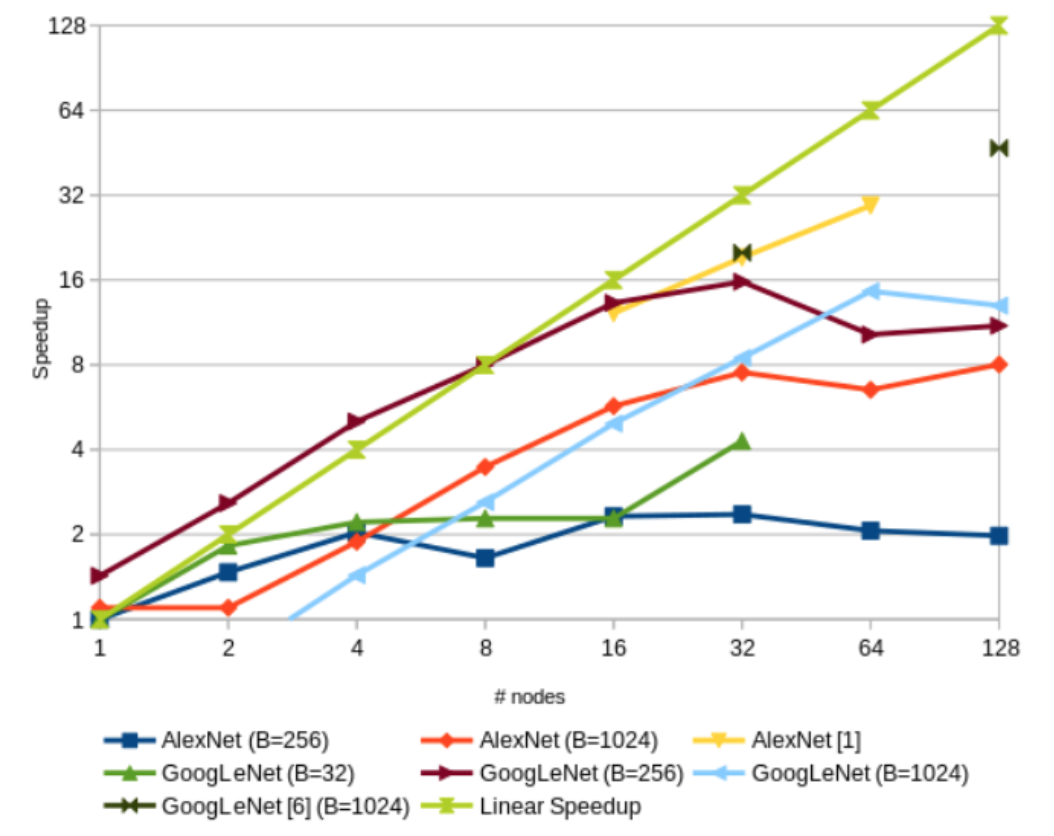
\includegraphics[width=1.0\linewidth]{img/speedup}}
\caption{Eperimental evaluation of DNN training scalability}
\label{fig:speedup1}
\end{center}
\vspace{-0.5cm}
\end{figure}


%%%%%%%%%%%%%%%%%%%%%%%%%%%%%%%%%%%%%%%%%%%
\section{Conclusions}
%%%%%%%%%%%%%%%%%%%%%%%%%%%%%%%%%%%%%%%%%%%
The research work presented in this paper explores the feasibility and efficiency of using Apache Spark and DL4J for 
deploying deep learning workloads over a real-world, petascale, HPC setup, such as MareNostrum.
To this end, we have designed a layered architecure consisting in both, general-purpose (Spark and DL4J) and custom components (Spark4MN). 
We have evaluated the deployment by training AlexNet and GoogLeNet over the ImageNet dataset. We have tested different deployment setups (number of nodes, number of Spark workers per node, data partition size, minibach size, averaging frequency, prefetching and repartitioning strategy).  

We conclude that it is feasible rely on Apache Spark to deploy deep learning workloads over a traditional HPC setup. This approach minimizes deployment costs and enables a systematic tuning of the different configuration parameters, both at application level and at infraestructure level. Nevertheless, a judicious configuration is necessary to achieve the proper scalability. The averaging frequency plays an important role and cannot be set too high or it may imply too networking overhead. The optimal setting is application dependent. Data locality and prefetching can be dismissed, as computation time will allways outweigh any network transfer time. The repartitioning strategy is also a [TODO: limits of synchronous data parallelism]


%%%%%%%%%%%%%%%%%%%%%%%%%%%%%%%%%%%%%%%%%%%
\section*{Acknowledgements}
%%%%%%%%%%%%%%%%%%%%%%%%%%%%%%%%%%%%%%%%%%%
This work is partially supported by the Spanish Ministry of Economy and Competitivity under contract TIN2015-65316-P and by the SGR programme (2014-SGR-1051) of the Catalan Government.

\begin{small}
\bibliographystyle{plain},
\bibliography{hpc,refs}
\end{small}

%\begin{IEEEbiography}[{\includegraphics[width=1in,height=1.25in,clip,keepaspectratio]{leonel_cruz.jpg}}]{Leonel Cruz}
%is a ... Contact him at ...
%\end{IEEEbiography}

%\begin{IEEEbiography}[{\includegraphics[width=1in,height=1.25in,clip,keepaspectratio]{ruben_tous.jpg}}]{Ruben Tous}
%is an associate professor in the Department of Computer Architecture at Universitat Polit\`ecnica de Catalunya. BarcelonaTech (UPC). His scientific work focuses on algorithms and data structures, knowledge representation and reasoning for multimedia understanding, multimedia databases and query languages, and %multimedia information retrieval. Tous has a PhD in computer science and digital communications from Universitat Pompeu Fabra, Spain. Contact him at rtous@ac.upc.edu.
%\end{IEEEbiography}

\end{document}
